\documentclass[a4paper,10pt,fleqn]{article} % Definiert Papier = A4;
%                                            % Schriftgrösse = 10Punkte;
%                                            % Mathe.-Gl. Modus = linksbündig
%                                            % (siehe http://lefti.amigager.de/latex/Aufbau.html)
%
\usepackage{../common/layout}

\newcommand{\myTitel}{Das Team 32}
\newcommand{\myDokumentTyp}{Teamvorstellung}
\begin{document}
    %
    % Deck- und Titelblatt
    %
    \begin{titlepage}
    \begin{center}
        \parindent0pt{\Huge\bfseries \myDokumentTyp}\\[0.5cm]
        {\huge PREN 1, Team 32}\\[1cm]
        Yves Studer\\
        Thomas Wiss\\
        Livio Kunz\\
        Niklaus Manser\\
        Matteo Trachsel\\
        Roger Gisler\\
        Pascal Roth\\
        \vspace*{1cm}
        {\Huge \myTitel}\\[0.5cm]
%        \begin{figure*}[h!]
%            \centering
%            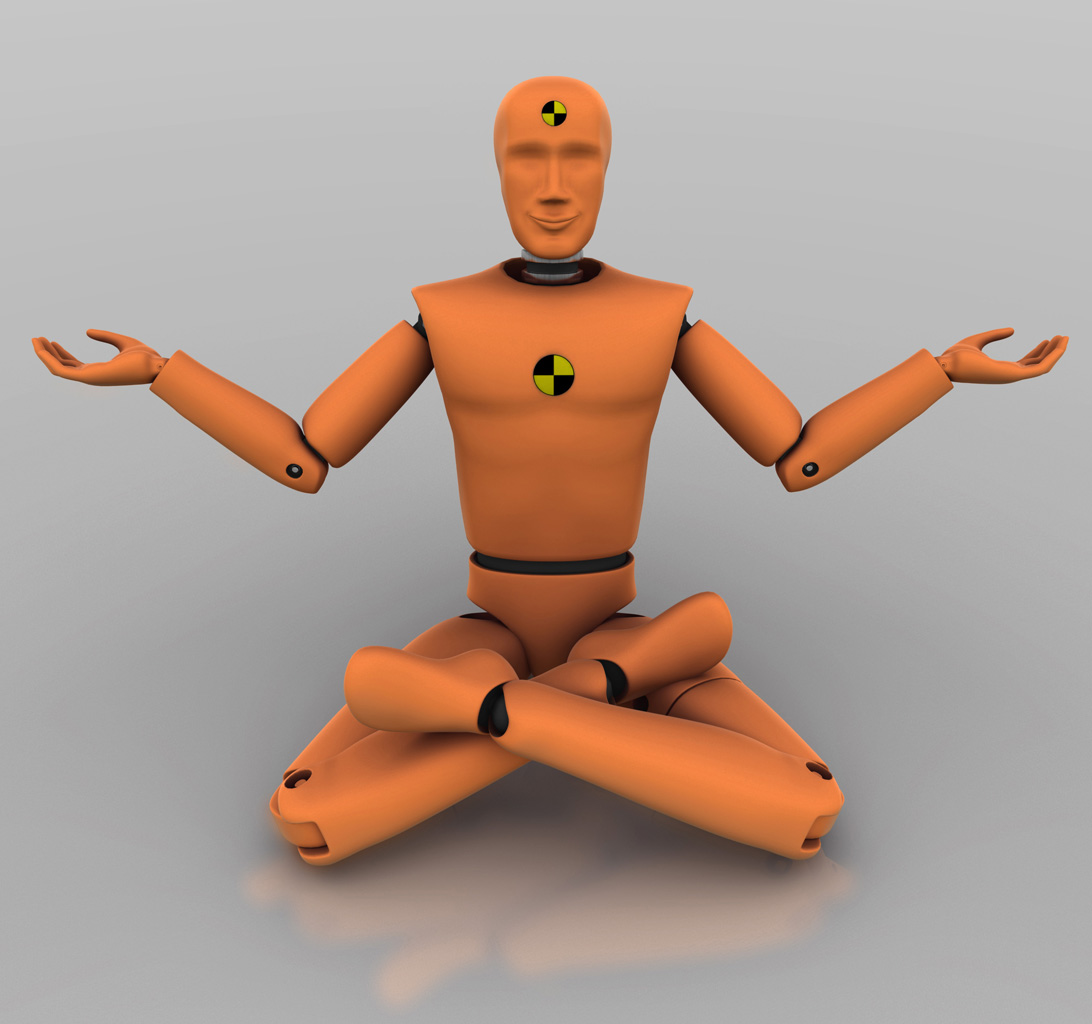
\includegraphics[width=0.7\textwidth]{Enddokumentation/Titelbild.JPG}
%        \end{figure*}
        
        \vfill{}
        {\normalsize Hochschule Luzern - Technik \& Architektur\\
         PREN 1}\\[0.6cm]
        {\normalsize Horw, Hochschule Luzern - T\&A, \today}
    \end{center}
\end{titlepage}

    \begin{titlepage}
    \begin{center}
        \parindent0pt{\Huge\bfseries \myDokumentTyp}\\[0.5cm]
		{\huge PREN 2, Team 32}\\[2em]
        \begin{tabular}{ll}
            Yves Studer                & Thomas Wiss \\
            Dorfstrasse 28             & Bachhüsliweg 4a \\
            6264 Pfaffnau              & 6042 Dietwil \\
            +41 79 705 48 88           & +41 79 604 93 61 \\
            yves.studer@stud.hslu.ch   & thomas.wiss@stud.hslu.ch \\
                                       & \\
            Livio Kunz                 & Niklaus Manser \\
            Hubelmatt 7                & Brunnmattstrasse 11\\
            6206 Neuenkirch            & 6010 Kriens \\
            +41 79 811 53 03           & +41 77 405 58 56 \\
            livio.kunz@stud.hslu.ch    & niklaus.manser@stud.hslu.ch \\
                                       & \\
            Matteo Trachsel			   & Roger Gisler \\
            Ogimatte 7                 & Eyrüti 16\\
            3713 Reichenbach           & 6467 Schattdorf\\
            +41 79 511 57 88           & +41 79 729 55 34 \\
            matteo.trachsel@stud.hslu.ch & roger.gisler@stud.hslu.ch \\
            						   & \\
            Pascal Roth			       & \\
            Dorfstrasse 18			   & \\
            6275 Ballwil		       & \\
            +41 79 717 68 94	       & \\
            pascal.roth@stud.hslu.ch   & \\
        \end{tabular}\\
        \vspace{3em}
        {\Huge \myTitel}\\[5em]
        Dozent: Markus Thalmann\\[2em]
        Hochschule Luzern - Technik \& Architektur\\   
        Interdisziplinäre Projektarbeit 2015
        \vfill{}
        Horw, Hochschule Luzern - T\&A, \today
    \end{center}
\end{titlepage}
    %
    % Inhlatsverzeichnis umbenennen und anschliessend einen Seitenumbruch
    %   
    \renewcommand{\contentsname}{Inhalt}
    \tableofcontents
    \newpage 
    %
    % Start mit der eigentlichen Arbeit
    %    
    %\label{sec:er}

\section{Personalblatt}
  \begin{tabular}{lp{3.3cm}l}
    Thomas Wiss                                 & &  \multirow{8}{4cm}{
\includegraphics[width=0.2\textwidth]{DasTeam/Bilder/ThomasWiss.jpg}} \\
    Bachhüsliweg 4a                             & &  \\
    6042 Dietwil                                & &  \\
    +41 79 604 93 61                            & &  \\
    Automatiker EFZ                             & &  \\
    thomas.wiss@stud.hslu.ch                 	& &  \\
    Studiengang: Informatik, Vollzeit           & &  \\
                                                & &  \\
                                                & &  \\
    Yves Studer                                 & &  \multirow{8}{4cm}{
\includegraphics[width=0.2\textwidth]{DasTeam/Bilder/YvesStuder.jpg}} \\
    Dorfstrasse 28                              & &  \\
    6264 Pfaffnau                               & &  \\
    +41 79 705 48 88                            & &  \\
    yves.studer@stud.hslu.ch                    & &  \\
    Multimediaelektroniker                      & &  \\
    Techniker HF, Elektrotechnik                & &  \\
    Studiengang: Elektrotechnik, Vollzeit       & &  \\
                                                & &  \\
    Livio Kunz                                  & &  \multirow{8}{4cm}{
\includegraphics[width=0.2\textwidth]{DasTeam/Bilder/LivioKunz.jpg}} \\
    Hubelmatt 7                                 & &  \\
    6206 Neuenkirch                             & &  \\
    +41 79 811 53 03                            & &  \\
    livio.kunz@stud.hslu.ch                     & &  \\
    Informatiker EFZ                            & &  \\
    Studiengang: Informatik, Vollzeit 			& &  \\
                                                & &  \\
                                                & &  \\
    Niklaus Manser                              & &  \multirow{8}{4cm}{
\includegraphics[width=0.2\textwidth]{DasTeam/Bilder/NiklausManser.jpg}} \\
    Brunnmattstrasse 11                         & &  \\
    6010 Kriens                                 & &  \\
    +41 77 405 58 56                            & &  \\
    niklaus.manser@stud.hslu.ch                 & &  \\
    Matura EFZ                    			    & &  \\
    Studiengang: Informatik, Vollzeit           & &  \\
                                                & &  \\
                                                & &  \\
    Matteo Trachsel                             & &  \multirow{8}{4cm}{
\includegraphics[width=0.2\textwidth]{DasTeam/Bilder/MatteoTrachsel.jpg}} \\
    Ogimatte 7                                  & &  \\
    3713 Reichenbach                            & &  \\
    +41 79 511 57 88                            & &  \\
    matteo.trachsel@stud.hslu.ch                & &  \\
    Matura                                      & &  \\
    Studiengang: Maschinenbau, Vollzeit         & &  \\
\end{tabular}
    
\begin{tabular}{lp{3.3cm}l}
    Roger Gisler                                & & 
	\multirow{8}{4cm}{
\includegraphics[width=0.2\textwidth]{DasTeam/Bilder/RogerGisler.jpg}} \\
    Eyrüti 16			                        & &  \\
    6467 Schattdorf                             & &  \\
    +41 79 729 55 34                            & &  \\
    roger.gisler@stud.hslu.ch                   & &  \\
    Polymechaniker                              & &  \\
    Studiengang: Maschinenbau, Vollzeit         & &  \\
                                                & &  \\
    				                            & &  \\
    Pascal Roth 								& & \multirow{8}{4cm}{
\includegraphics[width=0.2\textwidth]{DasTeam/Bilder/PascalRoth.jpg}} \\
    Dorfstrasse 18                              & &  \\
    6275 Ballwil                                & &  \\
    +41 79 717 68 94                            & &  \\
    pascal.roth@stud.hslu.ch                    & &  \\
    Automatiker                                 & &  \\
    Studiengang: Maschinenbau, Vollzeit         & &  \\
  \end{tabular}
    \newline
    \newline
    \newline
    %\label{sec:er}

\section{Teamcharta}

  Die Folgenden Punkte wurden mit dem ganzen Team erarbeitet. Dieses verbindliche Werk regelt den Umgang der einzelnen Teammitglieder untereinander. Wir wollen:

  \begin{itemize}
    \item Pünktlich sein
    \item Abmachungen/Termine einhalten und bei Problemen frühzeitig kommunizieren
    \item Probleme ansprechen und behandeln, nicht aussitzen
    \item Auch scheue Mitglieder einbeziehen
    \item Alle aussprechen lassen
    \item Arbeiten sorgfältig ausführen
    \item Entscheidungen gemeinsam ausdiskutieren
    \item Gegenseitiger Respekt
    \item Jedem Mitglied bei Problemen helfen
  \end{itemize}

    \section{Projektorganisation}
    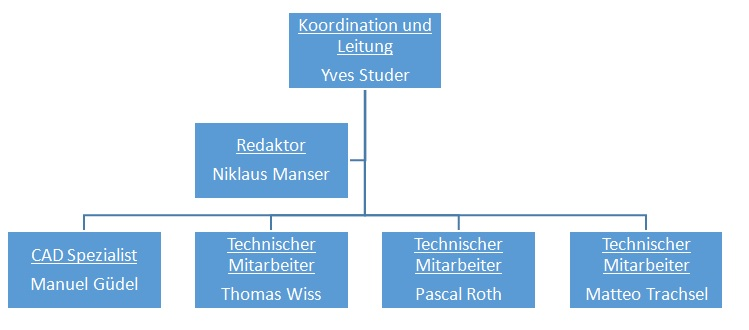
\includegraphics[width=1.05\textwidth]{DasTeam/Bilder/ProjektOrganisation.jpg}
    \section{Zielsetzung}
Im Team wurden die internen Ziele besprochen und wie folgt bestimmt. Die Aufzählung entspricht der Gewichtung:
\begin{enumerate}
\item Treffgenauigkeit
\item Geschwindigkeit
\item Gewicht
\end{enumerate}
Als optionales Ziel wurde beschlossen, dass das Gerät möglichst auch als Tennisballmaschine verwendbar (erweiterbar)
sein soll.\\
\\
\textbf{Weiter wollen wir die höchste Punktzahl erreichen!}

\end{document}
 No newline at end of file